%!TEX root = FDS_Technical_Reference_Guide.tex

\typeout{new file: Solid_Chapter.tex}

\chapter{Solid Phase} \label{SolidPhase}
\label{chapter:solid_phase}

FDS assumes that solid surfaces consist of multiple layers, with each layer composed of multiple material components that can undergo multiple thermal degradation reactions. Heat conduction is assumed only in the direction normal to the surface. Each reaction can produce multiple gas and solid species. This chapter describes the heat conduction equation for solid materials, plus the various coefficients, source terms, and boundary conditions, including the computation of the convective heat flux $\dq_{\rm c}''$ at solid boundaries.



\section{The Heat Conduction Equation for a Solid}

The one-dimensional heat conduction equation for the solid phase temperature $T_{\rm s}(x,t)$ is applied in the direction $x$ pointing into the solid (the point $x = 0$ represents the surface)\footnote{In cylindrical and spherical coordinates, the heat conduction equation is written
\be
  \rho_{\rm s} c_{\rm s} \; \dod{T_{\rm s}}{t} = \frac{1}{r} \, \dod{}{r}
  \left(r \, k_{\rm s} \dod{T_{\rm s}}{r} \right)+\dq_{\rm s}'''
  \quad ; \quad
  \rho_{\rm s} c_{\rm s} \; \dod{T_{\rm s}}{t} = \frac{1}{r^2} \, \dod{}{r}
  \left(r^2 \, k_{\rm s} \dod{T_{\rm s}}{r} \right)+\dq_{\rm s}'''
  \label{1dheatcyl}
\ee
FDS offers the user these options for cases where the obstruction surface is not flat, but rather cylindrical or spherical in shape. This option is useful in describing the behavior of small, complicated ``targets'' like cables or heat detection devices.}
\be
  \rho_{\rm s} c_{\rm s} \; \dod{T_{\rm s}}{t} = \dod{}{x} \left( k_{\rm s} \dod{T_{\rm s}}{x} \right) + \dq_{\rm s}'''
  \label{1dheat}
\ee
Section~\ref{matcoefs} describes the component-averaged material properties, $k_{\rm s}$ and $\rho_{\rm s} c_{\rm s}$. The source term, $\dq_{\rm s}'''$,
consists of chemical reactions and radiative absorption:
\be
  \label{eq:solid_energy_source_term}
  \dq_{\rm s}'''=\dq_{\rm s,c}'''+\dq_{\rm s,r}'''
\ee
Section~\ref{pyrosection} describes the term $\dq_{\rm s,c}'''$, which is essentially the heat production (loss) rate given by the  pyrolysis models for different types of solid and liquid fuels. Section~\ref{inradsection} describes the term $\dq_{\rm s,r}'''$, the radiative absorption and emission in depth.

The boundary condition on the front surface of a solid obstruction is
\be
 -k_{\rm s}\frac{\partial T_{\rm s}}{\partial x}(0,t) = \dot{q}_{\rm c}''+ \dot{q}_{\rm r}''
\ee
where $\dot{q}_{\rm c}''$ is the convective and $\dot{q}_{\rm r}''$ the radiative flux. If the radiation is assumed to penetrate in depth, the surface radiation term, $\dot{q}_{\rm r}''$, is set to 0. Section~\ref{conflux} describes the convective heat transfer to the solid surface.

On the back surface, there are two possible boundary conditions: (1) if the back surface is assumed to be open either to an ambient void or to another part of the computational domain, the back side boundary condition is similar to that of the front side, or (2) if the back side is assumed to be perfectly insulated, an adiabatic condition is used
\be
 -k_{\rm s}\frac{\partial T_{\rm s}}{\partial x} = 0
\ee
The numerical solution of the solid phase heat equation is presented in detail in Appendix~\ref{solid-phase-discretization}.

\subsection{Radiation Heat Transfer to Solids}
\label{inradsection}

If it is assumed that the thermal radiation from the surrounding gases is absorbed within an infinitely thin layer at the surface of the solid obstruction, then the net radiative heat flux is the sum of incoming and outgoing components, $\dq_{\rm r}'' = \dq_{\rm r,in}'' - \dq_{\rm r,out}''$:
\begin{align}
 \dq_{\rm r,in}'' &= \epsilon\,
 \int_{\bs'\cdot \bn_{\rm w} < 0} I_{\rm w}(\bs')\; |\bs'\cdot \bn_{\rm w} | \; \d\bO
 \label{RFluxIn1} \\[0.2in]
 \dq_{\rm r,out}'' &= \epsilon\,\sigma\,T_{\rm w}^4
 \label{RFluxOut1}
\end{align}
However, many common materials are not opaque; thus, the radiation penetrates the material to some finite depth. The radiative transport within the solid (or liquid) can be described as a source term in Eq.~(\ref{1dheat}). A ``two-flux'' model based on the Schuster-Schwarzschild approximation~\cite{Siegel:1} assumes the radiative intensity is constant inside the ``forward'' and ``backward'' hemispheres. The transport equation for the intensity in the ``forward'' direction is
\be
 \frac{1}{2}\frac{\d I^+(x)}{\d x}=\kappa_{\rm s}\,\left(I_{\rm b}-I^+(x)\right)
 \label{RInForward}
\ee
where $x$ is the distance from the material surface and $\kappa_{\rm s}$ is the component-averaged absorption coefficient:
\be
   \kappa_{\rm s} = \sum_{\alpha=1}^{N_{\rm m}} X_\alpha \; \kappa_{{\rm s},\alpha}
\ee
A corresponding formula can be given for the ``backward'' direction. Multiplying Eq.~\ref{RInForward} by $\pi$ gives us the ``forward'' radiative heat flux into the solid
\be
 \frac{1}{2}\frac{{\d\dq^+_{\rm r}(x)} }{\d x}=\kappa_{\rm s}\,
       \left(\sigma\,T_{\rm s}^4-\dq_{\rm r}^+(x)\right)
 \label{RFluxForward}
\ee
The radiative source term in the heat conduction equation is the sum of the ``forward'' and ``backward'' flux gradients
\be
  \dq_{\rm s,r}'''(x) = \frac{\d\dq_{\rm r}^+(x)}{\d x}+\frac{\d\dq_{\rm r}^-(x)}{\d x}
\ee
The boundary condition for Eq.~\ref{RFluxForward} at the solid (or liquid) surface is given by
\be
 \dq_{\rm r}^+(0) = \dq_{\rm r,in}'' + (1-\epsilon)\,\dq_{\rm r}^-(0)
 \label{RFluxInBC}
\ee
where $\dq_{\rm r}^-(0)$ is the ``backward'' radiative heat flux at the surface. In this formulation, the surface emissivity and the internal absorption are assumed constant.

The two-flux model has not been adapted for cylindrical or spherical geometry.

\subsection{Convective Heat Transfer to Solids}
\label{conflux}

The calculation of the convective heat flux depends on whether one is performing a direct numerical simulation (DNS) or a large eddy simulation (LES). For DNS, the convective heat transfer is calculated directly from the resolved gas and solid phase variables. For LES, there are a variety of empirical options.

\subsubsection{Direct Numerical Simulation}

In a DNS calculation, the convective heat flux to a solid surface $\dq''_{\rm c}$ is obtained directly from the gas temperature gradient at the boundary
\be
   \dq_{\rm c}'' = - k \; \dod{T}{n} = -k \frac{T_{\rm w}-T_{\rm g}}{\dn/2}
\ee
where $k$ is the thermal conductivity of the gas, $n$ is the spatial coordinate pointing into the solid, $\dn$ is the normal grid spacing, $T_{\rm g}$ is the gas temperature in the center of the first gas phase cell, and $T_{\rm w}$ is the wall surface temperature.

\subsubsection{Empirical Natural/Forced Convection Model}

In an LES calculation, the convective heat transfer coefficient, $h$, is based on a combination of natural and forced convection correlations:
\be \dq_{\rm c}'' = h \, (T_{\rm g} - T_{\rm w}) \quad \hbox{W/m}^2 \quad ; \quad
    h = \max \, \left[ \; C\, |T_{\rm g}-T_{\rm w}|^\ot \; , \;
    \frac{k}{L} \, \NU \; , \;
    \frac{k}{\dn/2} \right]  \quad  \si{W/(m^2.K)}
    \label{eq:qconv}
\ee
where $C$ is a empirical coefficient for natural convection (1.52 for a horizontal plate and 1.31 for a vertical plane or cylinder)~\cite{Holman:1}, $L$ is a characteristic length related to the size of the physical obstruction, and $k$ is the thermal conductivity of the gas. The Nusselt number (Nu) depends on the geometric and flow characteristics. For many flow regimes, it has the form:
\be
   \NU = C_1 + C_2 \, \RE^n \, \PR^m  \quad ; \quad \RE = \frac{\rho |\bu| L}{\mu} \quad ; \quad \PR = 0.7
\ee
For planar surfaces, the default values are $C_1=0$, $C_2=0.037$, $n=0.8$, $m=0.33$, and $L=1$~m. For cylindrical surfaces, the default values are $C_1=0$, $C_2=0.683$, $n=0.466$, $m=0.33$, and $L=D$, the diameter of the cylinder. For spherical surfaces, the default values are $C_1=2$, $C_2=0.6$, $n=0.5$, $m=0.33$, and $L=D$, the diameter of the sphere. Note that for a sphere, the coefficient for natural convection, $C$, is assumed to be zero. It is possible to change these values for a particular application, but it is not possible to find a set of parameters that is appropriate for the wide variety of scenarios considered. Various correlations for planes, cylinders, and spheres can be found in Refs.~\cite{Holman:1,Incropera:1}.


\subsubsection{Optional Near-Wall Model}
\label{conflux_wall_model}

This section describes an optional model for the heat transfer coefficient which may be more appropriate for well-resolved LES calculations.  This model has been validated for low Reynolds number heated channel flow \cite{Park:2012} and has been used in a model to predict upper layer temperature in airplane cargo compartments \cite{Oztekin:FM2012}.

Wall models aim to mimic the sudden change from molecular to turbulent transport close to the walls using algebraic formulations without resolving the smallest length scales. The theory follows dimensional analysis based on the idea that shear at the wall is constant. Accordingly, non-dimensional velocity can be defined as a function of non-dimensional length scale. In FDS, the wall model for velocity is implemented based on the law of the wall with a semi-log fit connecting the limits of the viscous and log regions (see Section~\ref{info:velocity_bc}).

By analogy to the near-wall model for velocity, the non-dimensional temperature is defined as
\begin{equation}
T^+ = \frac{T_{\rm g} - T_{\rm w}}{T_\tau}
\end{equation}
where $T_{\rm g}$ is the first off-wall gas-phase cell temperature.  The model profile is given by
\begin{align}
\label{eqn_t_visclayer} T^+ &= \mbox{Pr}\;y^+                            && \mbox{for} \quad y^+ \le 11.81 \\
\label{eqn_t_loglaw}    T^+ &= \frac{\mbox{Pr}_t}{\kappa} \ln y^+ + B_T  && \mbox{for} \quad y^+ \ge 11.81
\end{align}
where Pr and Pr$_{\rm t}$ are the molecular and turbulent Prandtl numbers  (Pr$_t=0.5$ by default in FDS), and $\kappa = 0.41$ is the von K\'arm\'an constant.  The temperature scale, $T_{\tau}$, is defined by
\begin{equation}
\label{eqn_friction_temperature}
T_{\tau} \equiv \frac{\dot{q}_{\rm c}''}{{\rho}{c_p}{u_{\tau}}}
\end{equation}
where $\dot{q}_{\rm c}''$, $\rho$, $c_p$ and $u_{\tau}$  are the convective heat flux at the wall, the gas density, the specific heat, and the friction velocity, respectively.

The second term, $B_T$, on the right hand side of Eq.~\ref{eqn_t_loglaw} is a function of the molecular Prandtl number and can be determined experimentally. Mathematically, this term is the integration constant stemming from the relation between velocity and temperature gradients. Physically, it represents the resistance to the heat and momentum transport close to the wall. FDS uses the experimental correlation proposed by Kader~\cite{Kader:1981}
\begin{align}
\label{eqn_t_bt}
B_T =(3.85 \,\mbox{Pr}^{1/3}-1.3)^2 + 2.12 \,\ln\mbox{Pr}
\end{align}
%The region $5 < y^+ < 30$ is referred to as the buffer layer.  In FDS, the buffer layer is approximated with a semi-log fit connecting the limits of the viscous and log regions
%\be
%\label{eqn_t_buffer_layer}
%T^+ = (\mbox{Pr}_t /\kappa)_{\rm buffer} \, \ln y^+ + B_{T,{\rm buffer}} \quad \mbox{for} \quad 5 < y^+ < 30
%\ee
%where
%\begin{align}
%(\mbox{Pr}_t /\kappa)_{\rm buffer} &= 1.79\,(B_T + 3.40 \,\mbox{Pr}_t - 5 \,\mbox{Pr}) \\[0.1in]
%B_{T,{\rm buffer}} &= 5 \,\mbox{Pr} - 1.61 \,(\mbox{Pr}_t /\kappa)_{\rm buffer}
%\end{align}
%To obtain a consistent convective heat transfer coefficient in all regions, $T^+$ is adjusted to $\max(T^+,T^+ (y^+ = 5))$ for the buffer and log layers ($y^+ \ge 5$).

The convective heat transfer coefficient ($h$) is obtained from the definition of $h$ and $T^+$:
\begin{align}
\label{eqn_h_model}
h = \frac{\dot{q}_{\rm c}''}{(T_{\rm g} - T_{\rm w})}= \frac{{\rho}{c_p}{u_{\tau}}}{T^+}
\end{align}


\subsection{Component-Averaged Thermal Properties}
\label{matcoefs}

The conductivity and volumetric heat capacity of the solid are defined as
\be
   k_{\rm s} = \sum_{\alpha=1}^{N_{\rm m}} X_\alpha \; k_{{\rm s},\alpha} \quad ; \quad
   \rho_{\rm s} c_{\rm s} = \sum_{\alpha=1}^{N_{\rm m}} \rho_{{\rm s},\alpha} \; c_{{\rm s},\alpha}
\ee
where $N_{\rm m}$ is the number of material components forming the solid, $X_\alpha$ is the volume fraction of component $\alpha$, and $\rho_{{\rm s},\alpha}$ is the {\em component density:}
\be
  \rho_{\rm s,\alpha}=\rho_{\rm s} \, Y_\alpha
\ee
where $\rho_{\rm s}$ is the density of the composite material and $Y_\alpha$ is the mass fraction of component $\alpha$. The solid density is the sum of the component densities
\be
  \rho_{\rm s} = \sum_{\alpha=1}^{N_{\rm m}} \rho_{\rm s,\alpha}
\ee
and the volume fraction of component $\alpha$ is computed as
\be
  X_\alpha = \frac{\rho_{\rm s,\alpha}}{\rho_\alpha}  \left/ \sum_{\beta=1}^{N_{\rm m}}\frac{\rho_{\rm s,\beta}}{\rho_{\beta} }  \right.
  \label{volfrac}
\ee
where $\rho_\alpha$ is the true density of material $\alpha$. Multi-component solids are defined by specifying the mass fractions, $Y_\alpha$, and densities, $\rho_\alpha$, of the individual components of the composite.


\subsection{Solid Heat Transfer 3D (Beta)}
\label{sec:ht3d}

This section describes the governing equations for heat transfer in the 3D solver, which may be implemented in FDS by setting {\ct HT3D=.TRUE.} on an {\ct OBST} line.  In-depth radiation may be treated using an optically thick approximation \cite{Modest:2003}, as discussed below.

Let $k_{\mathrm{s}}$, $\rho_{\mathrm{s}}$, and $c_{\mathrm{s}}$ denote, respectively, the thermal conductivity, density, and specific heat of the solid. The thermal properties may be functions of temperature.  The mean temperature of an Eulerian cell in the solid phase is denoted $T_{\mathrm{s}}$.  The heat flux vector is $\dot{\mathbf{q}}''$ and the volumetric heat source, either specified or from chemical reaction, is denoted $\dot{q}_{\mathrm{s}}'''$.  The governing equation for heat transfer is
\begin{equation}
  \rho_{\mathrm{s}} c_{\mathrm{s}} \; \dod{T_{\mathrm{s}}}{t} = - \Div\dot{\mathbf{q}}'' + \dot{q}_{\mathrm{s}}'''
  \label{eq:3dheat}
\end{equation}

\subsubsection*{Heat Flux}
\label{sec:heat_flux1}
{}
The intercell fluxes are continuous.  If the {\ct OBST} material properties of neighboring cells are the same, then thermal properties at face centers are taken as linear averages when computing the intercell flux. The intercell flux at time level $n$ may be obtained from either of the following (in practice the first relationship is used):
\begin{equation}
\label{eq:intercell_flux}
\dot{q}_{x,i+\frac{1}{2}}'' = - \left. k_{\mathrm{s}} \dod{T_{\mathrm{s}}}{x} \right|_{i+\frac{1}{2}} \approx - k_{{\mathrm{s}},i} \frac{T_{{\mathrm{s}},i+\frac{1}{2}}^n - T_{{\mathrm{s}},i}^n}{\frac{1}{2}\delta x_i} = - k_{{\mathrm{s}},i+1} \frac{T_{{\mathrm{s}},i+1}^n - T_{{\mathrm{s}},i+\frac{1}{2}}^n}{\frac{1}{2}\delta x_{i+1}}
\end{equation}

If the neighboring cells have different material properties (consider the $x$ direction with cell indices $i$ and $i+1$), then the cell interface temperature, $T_{s,i+\frac{1}{2}}$, is computed using
\begin{equation}
\label{eq:interface_tmp}
T_{{\mathrm{s}},i+\frac{1}{2}}^n = \frac{T_{{\mathrm{s}},i}^n + \left[\frac{k_{{\mathrm{s}},i+1}}{k_{{\mathrm{s}},i}} \frac{\delta x_i}{\delta x_{i+1}}\right] T_{{\mathrm{s}},i+1}^n}{1 + \left[\frac{k_{{\mathrm{s}},i+1}}{k_{{\mathrm{s}},i}} \frac{\delta x_i}{\delta x_{i+1}}\right]}
\end{equation}
which reduces to a simple linear average if $k_{{\mathrm{s}},i}=k_{{\mathrm{s}},i+1}$ and $\delta x_i=\delta x_{i+1}$.

\subsubsection*{Heat Flux with Local Material Deformation}
\label{sec:heat_flux2}

As a material shrinks or swells, the distance between material points decreases or increases.  It is challenging to handle this behavior on a static Eulerian grid.  Consider the situation depicted in Fig.~\ref{fig:flux_deform} where the material is shrinking.  As the temperature points move closer, the effect is to increase the intercell heat flux.  The flux becomes
\begin{equation}
\label{eq:fluxdef}
\dot{q}_{x,i+\frac{1}{2}}'' \approx - k_{i+\frac{1}{2}} \frac{ T_{s,i+1}-T_{s,i}}{\frac{1}{2}(\delta \tilde{x}_i + \delta \tilde{x}_{i+1})}
\end{equation}

\begin{figure}
\centering
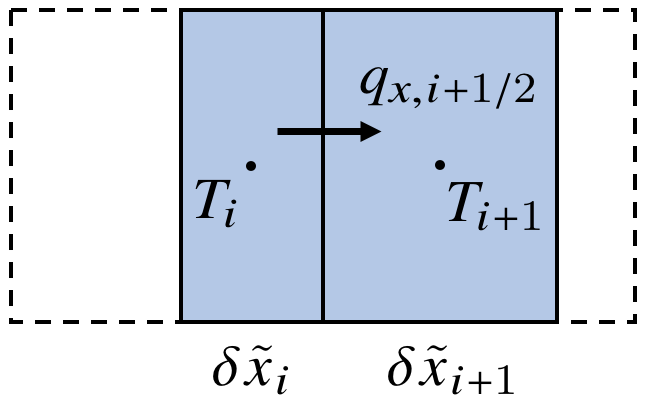
\includegraphics[height=1.25in]{FIGURES/flux_deform}
\caption{Diagram of intercell heat flux with a shrinking material.}
\label{fig:flux_deform}
\end{figure}

\noindent Calculation of the cell volumes, $\delta \tilde{x}$, etc., for pyrolysis with material deformation is discussed below.

\subsubsection*{Boundary Conditions}
\label{sec:boundary_conditions}

For two-way coupling between the gas and solid phase the boundary condition is continuity of heat flux and temperature.  On the gas phase side, the heat fluxes are due to convection and radiation, and on the solid phase side the heat flux is due to conduction.  The surface temperature links all these fluxes at an instant in time.  Let $T_{\mathrm{w}}$ denote the interface temperature between the gas and solid, the face temperature of the ``wall cell''.  The flux continuity boundary condition implies
\begin{equation}
\label{eq:fluxcontinuity}
\dot{q}_{{\mathrm{r}}, in}'' - \dot{q}_{{\mathrm{r}}, out}'' + \dot{q}_{\mathrm{c}}'' = -k_{\mathrm{s}} \left. \frac{\partial T_{\mathrm{s}}}{\partial n} \right|_{\mathrm{w}}
\end{equation}
To obtain the surface temperature, we take $\dot{q}_{{\mathrm{r}}, in}''$ from the radiation solver, linearize $\dot{q}_{{\mathrm{r}}, out}''$, and use Newton's law of cooling for $\dot{q}_{\mathrm{c}}''$. The flux condition may then be discretized as
\begin{equation}
\label{eq:discflux}
( \dot{q}_{{\mathrm{r}}, in}'' )^n + 3 \varepsilon^n \sigma \, (T_{\mathrm{w}}^n)^4 - 4 \varepsilon^n \sigma \, (T_{\mathrm{w}}^n)^3 \, T_{\mathrm{w}}^{n+1} + h^n (T_{\mathrm{g}}^n - T_{\mathrm{w}}^{n+1}) = -2 \, k_{\mathrm{s}}^n \, \frac{T_{\mathrm{s}}^n - T_{\mathrm{w}}^{n+1}}{\delta}
\end{equation}
where $T_{\mathrm{g}}$ is the gas temperature in the first off-wall grid cell and $n$ indicates the time level in the simulation.  Our result for the updated boundary temperature is
\begin{equation}
\label{eq:tmpwall}
T_{\mathrm{w}}^{n+1} = \frac{ ( \dot{q}_{{\mathrm{r}}, in}'' )^n + 3 \varepsilon^n \sigma \, (T_{\mathrm{w}}^n)^4 + h^n \, T_{\mathrm{g}}^n + 2 \, k_{\mathrm{s}}^n \, T_{\mathrm{s}}^n/\delta }{ 4 \varepsilon^n \sigma \, (T_{\mathrm{w}}^n)^3 + h^n + 2 \, k_{\mathrm{s}}^n / \delta}
\end{equation}

\subsubsection*{Surface Heat Flux Internal Wall Model}

In Eqs.~(\ref{eq:discflux}) and (\ref{eq:tmpwall}), the conductive heat flux into the wall is presumed to be resolved by a length scale, $\delta$.  In the 3D heat transfer model this length scale is \emph{not} taken to be the 3D cell spacing normal to the wall---the required 3D grid resolution would make the model intractable.  Instead, an internal wall model is employed.  To be consistent with the resolution of the 1D heat conduction model, the thermal penetration depth is taken to be
\begin{equation}
\label{eq:pendepth}
\delta = \sqrt{\frac{ \tau \; k_{\mathrm{s}}}{\rho_{\mathrm{s}} c_{\mathrm{s}}}}
\end{equation}
where $\tau$ is a somewhat arbitrary time scale set to unity.

% An alternate model for the thermal penetration depth that does not rely on an arbitrary time scale is
% \begin{equation}
% \label{eq:pendepth2}
% \delta = \left( \frac{\rho_{\mathrm{s}} \alpha_{\mathrm{s}}^3}{\dot{q}_w''} \right)^{1/3}
% \end{equation}
% where $\alpha_{\mathrm{s}} = k_{\mathrm{s}}/( \rho_{\mathrm{s}} c_{\mathrm{s}} )$.  Equation (\ref{eq:pendepth2}) is iterative since $\dot{q}_w''$ depends on $\delta$ (but convergence is very fast).  This length scale tends to be smaller than the depth given by Eq.~(\ref{eq:pendepth}).  The appropriate choice of length scale may be problem dependent.  Determining robust guidelines for grid independence of solid phase calculations is still an open area of research.  Presently, Eq.~(\ref{eq:pendepth2}) must be implemented at the source code level (there is no user hook).

\subsubsection*{Internal Radiation}
\label{sec:radiation}

The \emph{absorption coefficient} of the solid is denoted $\kappa_{\mathrm{s}}$.  If $\delta \times \kappa_{\mathrm{s}} \gg 1$, the material may be considered ``optically thick'' \cite{Modest:2003}.  This applies to many problems in pyrolysis.  The optically thick approximation implies a ``radiative conductivity'',
\begin{equation}
\label{eq:krad}
k_{\mathrm{r}} = \frac{16 n_{\mathrm{s}}^2 \sigma T_{\mathrm{s}}^3}{3 \kappa_{\mathrm{s}}} \,\mbox{,}
\end{equation}
which may simply be added to the material conductivity in the solver. Note that increasing the solid conductivity reduces the surface temperature, per Eq.~(\ref{eq:fluxcontinuity}), consistent with the notion that the radiation is not absorbed at the surface. Here, $n_{\mathrm{s}}$ is the material refractive index and $\sigma$ is the Stefan-Boltzmann constant.


\newpage
\section{Pyrolysis Models}
\label{pyrosection}

This section describes how solid phase reactions and the chemical source term in the solid phase heat conduction equation, $\dot{q}_{\rm s,c}'''$ (see Eq.~(\ref{eq:solid_energy_source_term})),  are modeled. This is commonly referred to as the ``pyrolysis model'', but it actually can represent any number of reactive processes, including evaporation, charring, and internal heating.


\subsection{Specified Heat Release Rate}

Often the intent of a fire simulation is merely to predict the transport of smoke and heat from a {\em specified} fire. In other words, the heat release rate is a specified input, not something the model predicts. In these instances, the desired heat release rate is translated into a mass flux for fuel at a given solid surface, which can be thought of as the surface of a burner:
\be
   \dm_{\rm f}'' = \frac{ f(t) \; \dq_{\rm user}''}{\Delta H_{\si{c}}}
\ee
Usually, the user specifies a desired heat release rate per unit area, $\dq_{\rm user}''$, plus a time ramp, $f(t)$, and the gas phase heat of combustion, $\Delta H_{\si{c}}$. The mass flux of fuel from the surface to the gas, $\dm_{\rm f}''$, can then be computed. A special subset of this approach is where the user also specifies a heat of combustion, density, and thickness for the burning material. If the default simple chemistry model described in Section~\ref{sec:simplechemistry}, with its single combustion reaction, is being used and there are multiple materials burning, one or more materials might have a different heat of combustion, $\Delta H_{\si{c}{\rm ,solid}}$, than the gas-phase combustion reaction. To account for this, FDS adjusts $\dm_{\rm f}''$ so that the solid phase has the appropriate mass loss rate, $\dm_{\rm f,solid}''$.
\be
\dm_{\rm f,solid}'' = \dm_{\rm f}'' \frac{\Delta H_{\si{c}}}{\Delta H_{\si{c}{\rm ,solid}}}
\ee

\subsection{Solid Fuels}

Solids can undergo simultaneous reactions under the following assumptions:
\begin{itemize}
\setlength{\itemsep}{0.0in}
\item instantaneous release of gas species
\item local thermal equilibrium between the solid and gaseous components
\item no condensation of gaseous products
\item no porosity effects\footnote{Although porosity is not explicitly included in the model, it is possible to account for it because the volume fractions defined by Eq.~(\ref{volfrac}) need not sum to unity, in which case the thermal conductivity and absorption coefficient are effectively reduced.}
\end{itemize}
Each material component may undergo several competing reactions, and each of these reactions may produce some other solid component (residue) and gaseous species according to specified yield coefficients.  These coefficients should sum to 1, but yields summing to less than 1 can account for products that are not explicitly included in the simulation.

The local density of material component $\alpha$ evolves in time according to the solid phase species conservation equation
\be
  \dod{ }{t} \left( \frac{\rho_{\rm s,\alpha}}{\rho_{\rm s}(0)} \right) =
    -\sum_{\beta=1}^{N_{\rm r,\alpha}} r_{\alpha \beta} + S_\alpha
  \label{solid_species_conservation}
\ee
where $N_{\rm r,\alpha}$ is the number of reactions for material $\alpha$, $r_{\alpha \beta}$ is the rate of reaction $\beta$ in units of \si{1/s},
and $\rho_{\rm s}(0)$ is the initial density of the material layer. $S_\alpha$ is the production rate of material component $\alpha$ as a result of
the reactions of the other components. The reaction rates are functions of solid and gas phase conditions and calculated as a combination of Arrhenius
and power functions:
\be
r_{\alpha \beta} =
    \underbrace{\left( \frac{\rho_{\rm s,\alpha}}{\rho_{\rm s}(0)}\right)^{n_{\rm s,\alpha\beta}}}_\textrm{Reactant dependency}
    \underbrace{A_{\alpha \beta} \; \exp \left(-\frac{E_{\alpha\beta}}{RT_{\rm s}}\right)}_\textrm{Arrhenius function}
    \underbrace{\left[X_{\rm O_2}(x)\right]^{n_{\rm O_2,\alpha\beta}}}_\textrm{Oxidation function}
    \underbrace{\max \big[0,S_{\rm thr,\alpha,\beta}(T_{\rm s}-T_{\rm thr,\alpha \beta}) \big]^{n_{\rm t,\alpha\beta}}}_\textrm{Power function}
   \label{Arrhenius}
\ee
The first term describes the dependence of the reaction rate on the concentration of the reactant itself, with $n_{\rm s,\alpha\beta}$ being the partial
reaction order. The second term is the Arrhenius function which is commonly used to describe the reaction kinetics, i.e. the dependence of the reaction
rate on the material temperature. The chapter on pyrolysis in the FDS Verification Guide describes methods for determining the kinetic parameters
$A_{\alpha \beta}$ and $E_{\alpha\beta}$ using bench-scale measurement techniques.

The third term can be used to describe the dependence on the
local oxygen concentration $X_{\rm O_2}(x)$ and the heterogeneous reaction order, $n_{\rm O_2,\alpha\beta}$.
The oxygen concentration profile within practical materials depends on the competition between diffusion and reactive consumption.
As FDS does not solve for the transport of gaseous species within condensed phase materials, a simple exponential profile is assumed and the
user is expected to specify the characteristic depth at which oxygen would be present.
The local oxygen volume fraction at depth $x$ is calculated from the gas phase (first grid cell) oxygen volume fraction $X_{\rm O_2,g}$ as
\be
X_{\rm O_2}(x) = X_{\rm O_2,g}\exp(-x/L_{\rm g,\alpha\beta})
\ee
where $L_{\rm g,\alpha\beta}$ is the characteristic depth of oxygen diffusion. Specifying $L_{\rm g,\alpha\beta}=0$ means that the reaction takes place
only at the surface of the material.

The fourth term is the power function where $T_{\rm thr,\alpha \beta}$ is a threshold temperature that can be used to dictate that the reaction must not occur below ($S_{\rm thr,\alpha,\beta}=+1$)  or above ($S_{\rm thr,\alpha,\beta}=-1$) a user-specified temperature. By default, the fourth term is deactivated ($S_{\rm thr,\alpha,\beta}=+1, T_{\rm thr,\alpha\beta}=0$ K).

Note that the solid species conservation equation~\ref{solid_species_conservation} and the reaction rate equation~\ref{Arrhenius} are inconsistent with the common practice of chemical kinetics convention, where the unit of the reaction rate is usually \si{kg/(m^3.s)} or \si{mol/(m^3.s)}. The current form can be obtained by dividing a more conventional reaction rate equation by $\rho_{\rm s}(0)$. This form is very close to the form used in \cite{Gpyro:FSJ} with the exception that initial layer density $\rho_{\rm s}(0)$ is used for scaling instead of the instantaneous value.

The production term $S_\alpha$ is the sum over all the reactions where the solid residue is material $\alpha$
\be
S_\alpha = \sum_{\alpha'=1}^{N_{\rm m}} \sum_{\beta=1}^{N_{\rm r,\alpha'}}
           \nu_{\alpha,\alpha' \beta} \; r_{\alpha' \beta}
       \quad \quad
           \hbox{(where Residue$_{\alpha' \beta}$ = Material$_\alpha$) }
\ee
where $\nu_{\alpha,\alpha' \beta}$ is the yield of component $\alpha$ from reaction $\beta$ of component $\alpha'$. The volumetric production rate of each gas species, $\gamma$, is
\be
\label{eq:pyrolyzate}
\dot{m}_{\gamma}''' = \rho_{\rm s}(0)\; \sum_{\alpha=1}^{N_{\rm m}} \sum_{\beta=1}^{N_{\rm r,\alpha}}
    \nu_{\rm \gamma,\alpha \beta} \; r_{\alpha \beta}
\ee
It is assumed that the gases are transported instantaneously to the surface, where the
mass fluxes are given by\footnote{In cylindrical and spherical coordinates, the mass fluxes are
\be
   \dm_\gamma'' =\frac{1}{R_{\rm out}}   \int_{R_{\rm in}}^{R_{\rm out}} \dm_\gamma'''(x) \,r \d r \;\; ; \;\;
   \dm_\gamma'' =\frac{1}{R_{\rm out}^2} \int_{R_{\rm in}}^{R_{\rm out}} \dm_\gamma'''(x) \,r^2 \d r \;\;
\ee}
\be
\label{eq:1dmassflux_solid}
\dm_\gamma'' = \int_0^L \dm_\gamma'''(x) \,\d x
\ee
where $L$ is the thickness of the solid. The chemical source term in the heat conduction equation is
\be
\label{eq:qchem_solid}
\dot{q}_{\rm s,c}'''(x) = -\rho_{\rm s}(0)\; \sum_{\alpha=1}^{N_{\rm m}} \sum_{\beta=1}^{N_{\rm r,\alpha}}  r_{\alpha \beta}(x) H_{\rm r,\alpha \beta}
\ee
where $H_{\rm r,\alpha \beta}$ is the heat of reaction.

\subsection{Phase Change Reactions}

To describe freezing or melting of liquids, the two phases are separated by a sharp interface at the constant phase-change temperature, $T_{\rm f}$. The location of the phase boundary $x_{\rm f}$ is governed by the equation
\be
k_{\rm s,1} \dod{T_{\rm s,1}}{x}-k_{\rm s,2}\dod{T_{\rm s,2}}{x} = \rho_{\rm s} H_{\rm r,\alpha\beta} \dod{x_{\rm f}}{t}
\ee
where 1 and 2 refer to the materials on the two sides of the boundary. In the context of the fixed-grid finite-difference method, it is more convenient
to allow a small deviation from $T_{\rm f}$ and solve for the amount of mass reacting during the time step, $\Delta t$,
from the energy required to convert the mass from one phase to the other
\be
\dot{m}''' \Delta t = \frac{\rho_{\rm s} c_{\rm s}(T_{\rm s}-T_{\rm f})}{H_{\rm r,\alpha\beta}}
\ee
This reaction can be implemented by setting $T_{\rm thr,\alpha\beta} = T_{\rm f}$ and $A_{\alpha\beta} = c_{\rm s}$ and turning on a specific
{\em phase-change reaction} mode. The reaction rate given by Eq.~\ref{Arrhenius} is then divided by the factor $H_{\rm r,\alpha\beta} \Delta t$.

\subsection{Liquid Fuels}

The rate at which liquid fuel evaporates when burning is a function of the liquid temperature and the concentration of fuel vapor above the pool surface. According to the Clausius-Clapeyron relation, the volume fraction of the fuel vapor above the surface is a function of the liquid boiling temperature
\be X_{\rm F,\ell} = \exp \left[ -\frac{ h_{\rm v} W_{\rm F}}\R \left(\frac{1}{T_{\rm s}}-\frac{1}{T_{\rm b}} \right) \right]
\label{CC_liquid}
\ee
where $h_{\rm v}$ is the heat of vaporization, $W_{\rm F}$ is the molecular weight of the fuel gas, $T_{\rm s}$ is the surface temperature, and $T_{\rm b}$ is the boiling temperature of the fuel~\cite{Prasad:1}. The evaporation rate of the fuel is governed by Stefan diffusion~\cite{Taylor&Krishna}:
\be
\dot{m}'' = h_{\rm m} \; \frac{\bp_m W_{\rm F}}{\R T_{\rm g}} \; \ln \left(\frac{X_{\rm F,g}-1}{X_{\rm F,\ell}-1}\right) \quad ; \quad h_{\rm m}= \frac{\SH \, D_{\rm \ell,g}}{L}
\ee
where $\bp_m$ is the pressure, $T_{\rm g}$ is the temperature, and $X_{\rm F,g}$ is the volume fraction of fuel vapor in the grid cell adjacent to the pool surface. The Sherwood number is given by
\be
\SH=0.037~\SC^{\frac{1}{3}} \RE^{\frac{4}{5}} \quad ; \quad {\rm Sc}=0.6 \quad ; \quad \RE= \frac{\rho~||\bu||~L}{\mu}
\ee
The Reynolds number is calculated based on conditions in the cell adjacent to the surface. The length scale, $L$, used in calculating the Reynolds number is \SI{1}{m} unless otherwise specified and is the same length scale used for the convective heat transfer calculation.

For simplicity, the liquid fuel itself is treated like a thermally-thick solid for the purpose of computing the heat conduction. There is no computation of the convection of the liquid within the pool.

\subsection{Shrinking and Swelling Materials}
\label{sec:shrink_swell}

The layer thickness is updated according to the ratio of the instantaneous material density and the density of the material in its pure form. In case of several material components, the amount of swelling and shrinking is determined by the maximum and sum of these ratios, respectively. In each time step, the size of each condensed phase cell is multiplied by the following factor:
\be
\delta =
   \begin{cases}
   \max_{\alpha}\left(\frac{\rho_{\rm s,\alpha}}{\rho_\alpha}\right) & \text{if }\max_{\alpha}\left(\frac{\rho_{\rm s,\alpha}}{\rho_\alpha}\right) \geq 1 \\
   \sum_{\alpha}\left(\frac{\rho_{\rm s,\alpha}}{\rho_\alpha}\right) & \text{if }\max_{\alpha}\left(\frac{\rho_{\rm s,\alpha}}{\rho_\alpha}\right) < 1
   \end{cases}
\ee
Correspondingly, the densities are divided by the factor $\delta$ to conserve mass.

\subsection{Solid Pyrolysis 3D (Beta)}

To begin our discussion of pyrolysis it is useful to start with definitions of the material mass density and volume.  We consider a solid composed of a mixture of material components $\alpha$.  The \emph{material density} (a property of the material) is
\begin{equation}
\label{eq:matden}
\rho_\alpha \equiv \frac{m_\alpha}{V_\alpha}
\end{equation}
The \emph{bulk density} is
\begin{equation}
\label{eq:bulkden}
\rho_{\mathrm{s},\alpha} \equiv \frac{m_\alpha}{V_{\mathrm{s}}}
\end{equation}
And the \emph{total solid density} is
\begin{equation}
\label{eq:totalsolidden}
\rho_{\mathrm{s}} \equiv \sum_\alpha \rho_{\mathrm{s},\alpha}
\end{equation}

The reaction kinetics and heat source terms are the same in 1D and 3D.  The bulk density of material component $\alpha$ evolves by Eq.~(\ref{solid_species_conservation}) and the chemical heat source term is given by Eq.~(\ref{eq:qchem_solid}).

\subsubsection*{Local Material Deformation}
\label{sec:locmatdef}

A discussion about how the 1D model handles shrinking and swelling materials can be found in Sec.~\ref{sec:shrink_swell}.  In this section, we deal with the same issue in 3D.  One of the key differences in the 1D and 3D models is that the concept of ``thickness'' in the 1D model is not dependent at all on the 3D computational mesh.  In the 1D solver, the material shrinks from the bottom up, with the face of the solid stationary (until the cell potentially burns away).

Conversely, in 3D the solid mass is tied to the Eulerian grid cell.  The grid cell itself cannot disappear.  Instead we track the solid volume relative to the local cell volume.  This volume ratio may be computed from the material densities as follows:
\begin{equation}
\label{eq:volratio}
\phi_{\mathrm{s}} \equiv \frac{V_{\mathrm{s}}}{V_{\mathrm{cell}}} = \frac{\sum_\alpha V_\alpha}{V_{\mathrm{cell}}} = \sum_\alpha \frac{m_\alpha/\rho_\alpha}{m_\alpha/\rho_{\mathrm{s},\alpha}} = \sum_\alpha \frac{\rho_{\mathrm{s},\alpha}}{\rho_\alpha}
\end{equation}

We presently consider two simple models for material deformation: isotropic and unidirectional.  The method is based on the definition $V_{\mathrm{s}}= \phi_{\mathrm{s}} V_{\mathrm{cell}}$, which is equivalent to $\prod_i \delta \tilde{x}_i = \phi_{\mathrm{s}} \prod_i \delta x_i$. For a 2D case, if the material deforms equally in both directions (isotropic) then the spacing used to compute heat fluxes is computed from
\begin{align}
\label{eq:dxdefiso}
\delta \tilde{x} &= \phi_{\mathrm{s}}^{1/2} \delta x \nonumber\\
\delta \tilde{y} &= \phi_{\mathrm{s}}^{1/2} \delta y
\end{align}

If, on the other hand, we have a preferred direction for mass loss (such as in a cone calorimeter test), then the deformation is considered unidirectional.  The flux spacing is computed as (deformation in $x$)
\begin{align}
\label{eq:dxdefuni}
\delta \tilde{x} &= \phi_{\mathrm{s}} \delta x \nonumber\\
\delta \tilde{y} &= \delta y
\end{align}

\subsection{Mass Transport}
\label{sec:mass_transport}

The movement of pyrolysis gas through the material to the solid surface is complicated to model in detail.  In many practical codes, mass transfer resistance is simply ignored.  Thus, any gas generated via pyrolysis is imagined to instantaneously appear at the solid surface as a mass flux boundary condition to the gas phase.  The 3D model allows both instantaneous transport and diffusive transport, which we discuss below.

\subsubsection*{Gas Generation}
\label{eq:gas_generation}

Similar to Eq.~(\ref{eq:pyrolyzate}), in 3D the mass generation rate per unit volume of pyrolysis gas component $\gamma$ in cell $i,j,k$ is given by
\begin{equation}
\label{eq:massprod}
\dot{m}_{\gamma,i,j,k}''' = \rho_{\mathrm{s}}(0)_{i,j,k} \sum_{\alpha=1}^{N_{\mathrm{m}}} \sum_{\beta=1}^{N_{\mathrm{r},\alpha}} \nu_{\gamma,\alpha\beta} r_{\alpha\beta,i,j,k}
\end{equation}

\subsubsection*{Instantaneous Transport}
\label{sec:instantaneous_transport}

Similar to the 1D model, instantaneous transport is the default mode of operation in the 3D model.  However, implementation is not as straight-forward in 3D since Eulerian cells more than one cell below the surface are not usually tied to a ``wall cell''.  In 3D, unless the user specifies otherwise, mass is ejected via the nearest wall cell and the deformation model is taken to be isotropic.  Alternatively, the user may specify the direction for mass ejection and the deformation model becomes unidirectional.

For instantaneous transport, the mass flux at the solid surface for a given wall cell is the summation of the mass production in the column of solid cells tied to the wall cell.  For a column of cells in the $z$ direction tied to wall cell $w$, we have
\begin{equation}
\label{eq:mdotint}
\dot{m}_{\gamma,w}'' = \sum_{k \in w} \dot{m}_{\gamma,i,j,k}''' \,\delta z_k
\end{equation}
This is the 3D discrete analog of Eq.~(\ref{eq:1dmassflux_solid}).

\subsubsection*{Diffusive Transport}
\label{sec:diffusive_transport}

A less arbitrary way to assign the pyrolysis gas to a wall cell is to simply solve a transport equation.  While the physics is not so simple in reality, an isotropic diffusion model of transport has several advantages:  It is easy to implement.  It avoids any ad hoc assumptions applied in the instantaneous model.  It handles smoldering combustion and char oxidation naturally.  And finally, while the physics are not perfect, they are usually qualitatively correct and the implementation lends itself to improvement.

The diffusive transport equation for gas component $\gamma$ is given by
\begin{equation}
\label{eq:diff}
\frac{\partial \rho_\gamma}{\partial t} = - \Div\mathbf{J}_\gamma + \dot{m}_{\gamma}'''
\end{equation}
where the diffusive flux is modeled with Fick's law,
\begin{equation}
\label{eq:fick}
\mathbf{J}_\gamma = - D_{\gamma} \tilde{\nabla} \rho_\gamma
\end{equation}
Note that the gradient operator is written in terms of a deformed space coordinate, in the same manner as the heat flux.  In the current implementation, the diffusivity is isotropic.  The default is the gas phase molecular value for component $\gamma$.  However, the user may adjust this value if needed.

\subsubsection*{Transport Boundary Conditions}
\label{sec:transport_bcs}

Consider the flux between solid cell $i$ and gas phase cell $i+1$.  The surface is denoted by F for ``face value''. The mass flux at the solid surface is taken from
\begin{equation}
\label{eq:massflux_boundary}
J_{\gamma,\mathrm{F}} = - D_{\gamma,\mathrm{F}} \frac{\rho_{\gamma,\mathrm{F}} - \rho_{\gamma,i}}{\frac{1}{2}\delta \tilde{x}_i}
\end{equation}
where
\begin{equation}
\label{eq:rhoF}
\rho_{\gamma,\mathrm{F}} =
\left\{\begin{array}{ll}
0                          & \mbox{if $\gamma$ is fuel} \\
\rho Y_{\gamma,\mathrm{F}} & \mbox{if $\gamma$ is oxidizer} \\
\rho_{\gamma,i}            & \mbox{if boundary is impermeable, $J_{\gamma,\mathrm{F}}=0$}
\end{array}\right.
\end{equation}

The boundary conditions in Eq.~(\ref{eq:rhoF}) provide qualitatively correct behavior for the pyrolysis gases (transport \emph{out} of the solid) while allowing diffusion of oxidizer into the solid.  Using $\rho Y_{\gamma,\mathrm{F}}$ for the fuel can lead to erratic behavior caused by diffusion of fuel back into the solid, which is not physical.  This ad hoc treatment of the boundary is a limitation of the diffusion model, but we note that the scheme is no worse than the instantaneous transport out of the solid used in most 1D models.

It should be noted that $\rho Y_{\gamma,\mathrm{F}}$ is currently taken from the gas phase solver at the current time level.  The mass flux is therefore time lagged between the gas phase and solid phase solvers, unlike the surface temperature from Eq.~(\ref{eq:tmpwall}).  This is a potential source of error that will be addressed in future development.


\newpage
\section{Aerosol Deposition}

By default, FDS assumes that soot is transported just like all other gaseous species. That is, the soot particles are small enough that their settling velocity is small compared to the fire-driven flows of the gas containing the soot. Near surfaces, however, other mechanisms can affect the soot, which results in its deposition onto surfaces. The removal of soot via deposition can impact the visibility for egress and the time for smoke detectors to activate. In forensic fire reconstructions, the amount of soot deposited on surfaces can be correlated to post-fire observations. The deposition of particulates is also important for computing the dispersion characteristics of aerosol toxicants like ash, radionuclides, or other particulate matter.

However, there is an option to treat any gas phase species as an aerosol that can be deposited on surfaces. Aerosol deposition is determined by applying an empirical deposition velocity to aerosols near surfaces. There are a number of phenomena that cause deposition: thermophoresis (where temperature gradients push the aerosol towards or away from the surface), gravitational settling, diffusive deposition (where the aerosols move along the boundary layer concentration
gradient), and turbulent deposition (essentially impact deposition due to a turbulent boundary layer). Other phenomena, such as electrical fields, can also result in deposition but are not considered in FDS due to their relatively small contribution in compartment fire scenarios.

The total aerosol deposition velocity to surfaces, $u_{\rm dep}$, is determined by assuming the deposition phenomena are independent, computing a deposition velocity for each mechanism, and then summing them~\cite{Bixler:1}
\be
u_{\rm dep} = u_{\rm g}+u_{\rm th}+u_{\rm dt}
\ee
where $u_{\rm g}$ is the gravitational settling velocity (for cells near upward-facing surfaces), $u_{\rm th}$ is the thermophoretic velocity, and $u_{\rm dt}$ is the combined diffusion-turbulence velocity. If the aerosol is located in a gas-phase cell adjacent to a wall, then the aerosol (represented by the subscript $\alpha$) is removed from the gas-phase and deposited onto the surface by imposing the following boundary condition
\be
\dot m_{\rm dep,\alpha}'' = \rho Y_\alpha \, u_{\rm dep}
\ee
Using this boundary condition, the aerosol surface density that accumulates on surfaces is tracked, and the amount
of aerosol that deposits to a surface is removed from the adjacent gas-phase cell.
Note that the subscript $\alpha$ refers to a species that contains soot or aerosol, whereas the subscript `a'
in the remainder of the section refers to the condensed phase soot or aerosol properties, such as mass or density.

\subsection{Gravitational Settling}

The gravitational settling velocity is given by~\cite{Davies_Charles}
\be
u_{\rm g} = g m_{\rm a} \frac{\text{Cn}}{6 \pi \, \chi_{\rm d} \, \mu \, r_{\rm a}}
\ee
where $m_{\rm a}$ is the particle mass, $\chi_{\rm d}$ is a shape factor, $\mu$ is the dynamic viscosity of air,
$r_a$ is the particle radius, and Cn is the Cunningham slip correction factor given by~\cite{Davies_Charles}
\be
\text{Cn} = 1 + 1.257 \; \text{Kn} + 0.4 \; \text{Kn} \; \mathrm{e}^{-1.1/\text{Kn}}
\ee
where Kn is the particle Knudsen number given by the ratio of the mean free path of the gas
to the particle radius. Kn is computed as~\cite{Sippola:1}
\be
\text{Kn} = \frac{\lambda}{r_{\rm a}}
\ee
where $\lambda$ is the mean free path of gas molecules which is computed as~\cite{Jennings_S_G}
\be
\lambda = \mu_g \; \sqrt {\frac {\pi}{2 \; p \; \rho_g} }
\ee
For each aerosol species in the gas phase, a gravitational settling velocity is calculated
and imposed on the convective term in the species transport
equation~(Eq.~\ref{species}). This approach is similar to the drift flux model
for smoke transport described in Hu et al.~\cite{Hu:1}. The gravitational settling velocity
is also included in the total deposition velocity to deposit aerosols onto upward-facing flat surfaces,
as described above.


\subsection{Thermophoretic Deposition}

The thermophoretic velocity is computed as
\be
u_{\rm th} = \frac{K_{\rm th} \nu}{T_{\rm g}} \; \frac{\d T}{\d x}
\ee
This requires the wall temperature gradient, which is only resolved in a DNS simulation.
For an LES simulation, the temperature gradient is computed from the wall heat transfer coefficient.
\be
 \frac{\d T}{\d x} = \frac{h \left( T_{\rm g} - T_{\rm w} \right)}{k_{\rm g}}
\ee
$K_{\rm th}$ is the thermophoretic velocity coefficient and is calculated using the following correlation~\cite{Brock:1}
\be
 K_{\rm th} = \frac{2 \, C_{\rm s} \left(\alpha + C_{\rm t} \; \text{Kn} \right) \; \text{Cn}}{\left(1 + 3 \, C_{\rm m} \; \text{Kn} \right) \left(1 + 2 \, \alpha + 2 \, C_{\rm t} \, \text{Kn} \right) }
\ee
where $C_{\rm s}=1.17$ is the thermal slip coefficient, $\alpha$ is the ratio of the gas
conductivity to the particle conductivity, $C_{\rm m}=1.14$ is the momentum accommodation
coefficient, and $C_{\rm t}=2.18$ is the thermal accommodation coefficient.

For each aerosol species in the gas phase, a thermophoretic velocity is calculated and imposed on the convective term in the species transport equation~(Eq.~\ref{species}). This approach follows the drift flux model
for smoke transport described in Hu et al.~\cite{Hu:1}.

\subsection{Turbulent Deposition}

The diffusion-turbulence deposition velocity depends upon the flow regime
(diffusion, diffusion-impaction, or inertia-moderated). The deposition velocity
for these regimes is given below~\cite{McCoy_Hanratty}.
\be
u_{\rm dt} = \left\{ \begin{array}{r@{\quad \quad}l}
         0.086 \; \text{Sc}^{-0.7} \; u_{\tau}        &  \tau^+ < 0.2 \\
         3.5 \times 10^{-4} \; {\tau^+}^2 \; u_{\tau} &  0.2 < \tau^+ < 22.9 \\
         0.17 \; u_{\tau}                             &  \tau^+ > 22.9
         \end{array} \right.
\ee
where Sc is the particle Schmidt number, or the ratio of the kinematic viscosity to the
Brownian diffusion coefficient of the particle ($\nu/D_{\rm B}$), $u_{\tau}$ is the wall friction velocity
computed by the wall model, and $\tau^+$ is the dimensionless stopping distance given by~\cite{Ludwig_ICONE}
\be
 \tau^+=\frac{\rho_{\rm a} \, (2 r_{\rm a})^2}{18 \, \mu^2}  \; u_{\tau}^2 \; \rho_{\rm g}
\ee

\newpage
\section{Aerosol Agglomeration}

Agglomeration is the process via which small aerosol particles become larger aerosol particles due to collisions that cause the smaller particles to stick together and become larger particles. The FDS implemenation of aerosol agglomeration is based on the agglomeration model in VICTORIA~\cite{NRC:VICTORIA}, a US NRC software package for modeling radioactive aerosol transport during severe accidents. The agglomeration mechanisms in FDS include Brownian, graviational, and turbulent (sheer and inertial). The agglomeration is governed by the equation below.
\be
\frac{\d N}{\d t} = \frac{1}{2} \int_{0}^{m} \Phi (\omega,m-\omega) N(\omega) N(m-\omega) \d \omega - N(m) \int_{0}^{\infty} \Phi (\omega,m) N(\omega) \d \omega - R(m) + S(m)
\ee
In the above equation $\Phi$ is an agglomeration kernel, $N(m)$ is the number density of particles of size $m$, $R$ is a removal term (e.g. outflow, oxidation), and $S$ is a source term (e.g. from combustion). The equation states that the rate of formation of particles of size $m$ is the rate that two particles whose combined size is $m$ collide, minus the rate at which particles of size $m$ collide with other particles and become a larger size, minus removal of particles of size $m$, and plus the generation of particles of size $m$. The selected approach for solving the agglomeration equation is to bin the particle sizes into multiple bins and transform the integrals over particle size into summations over particle bins. By defining the maximum, $m_{max}$, and minimum, $m_{min}$, particle mass and the number of bins, $M$, one can define the average bin mass, $x$, as shown below~\cite{Higgins_Davidson}.
\be
s = \left( \frac{m_{max}}{m_{min}} \right) ^{1/M} \; , \; m_i =s \; m_{i-1} \; , \; x_i = \frac{2 m_i}{1+s}
\ee
Using this binning, the agglomeration equation becomes:
\be
\frac{\d N_i}{\d t} = \sum_{k=1}^{M} \sum_{j=k}^{M} \left( 1- \frac{1}{2} \delta_{j,k} \right) \eta \Phi(j,k) N_j N_k - N_i \sum_{k=1}^M \Phi(j,k) N_k - R_i + S_i
\ee
where $\eta$, shown below, is a function for apportioning mass between adjacent particle bins.
\be
\eta = \begin{cases}
	\frac{x_{i+1}-m_i}{x_{i+1}-x_i} & x_i< m_i \leq x_{i+1} \\
    \frac{m_i-x_{i-1}}{x_i-x_{i-1}} & x_{i-1}< m_i \leq x_i
	\end{cases}
\ee
The agglomeration kernel is given by the sum of the Brownian (Br), gravitational (Gr), shear (Sh), and inertial (In) agglomeration  terms.
\be
\Phi (m,\omega)= \Phi_{\rm Br}(m,\omega) + \Phi_{\rm Gr}(m,\omega) + \sqrt{\Phi_{\rm Sh}(m,\omega)^2 + \Phi_{\rm In}(m,\omega)^2}
\ee
Browian agglomeration occurs when the random walks of particles brings them into contact with one another. It is computed as~\cite{NRC:VICTORIA}:
\be
\Phi_{\rm Br}= 4 \pi k_{\rm b} T \left({\rm B} (m) + {\rm B} (\omega) \right) \left(r_m+r_{\omega} \right) {\rm Fu} (m,\omega)
\ee
where Fu is the Fuchs factor and B is the particle mobility.
\be
{\rm B}(m) = \frac {\rm Cn}{6 \pi \mu r_m}
\ee
\be \frac{1}{{\rm Fu}(m,\omega)} = \left( \epsilon_s \frac{r_m + r_{\omega}}{k_{\rm b} T \left({\rm B}(m) + {\rm B}(\omega) \right)} \sqrt {\frac{8 k_{\rm b} T}{\pi} \left(\frac{1}{m}+\frac{1}{\omega} \right)} \right)^{-1} +
	\left( 1+\frac{2 \sqrt{(\tilde{a}_m^2+\tilde{a}_{\omega}^2)}}{r_m+r_{\omega}} \right)^{-1}
\ee
\be
\tilde{a}_m = \frac { \left(r_m + a_m \right)^3 - \left(r_m^2 + a_m^2 \right)^{3/2}} {3 r_m a_m} - r_m
\ee
\be
a_m= {\rm B} (m) \sqrt{ \frac{2 k_{\rm b} T m} {\pi}}
\ee
Gravitational agglomeration results from heavier particle falling onto larger particles. The efficiency of these collisions are governed by a sticking factor, $\epsilon_{\rm S}$ assumed to be one, and a collision efficiency, $\epsilon_{\rm PK}$~\cite{NRC:VICTORIA}
\be
\Phi_{\rm Gr} (m,\omega) = \epsilon_{\rm S} \epsilon_{\rm PK}(m,\omega) \left(r_m+r_{\omega} \right)^2 \left| u_g(m)-u_g(\omega) \right|
\ee
\be
\epsilon_{\rm PK}(m,\omega) = \frac {{\rm min} \left(r_m,r_{\omega} \right)^2}{2 \left( r_m+r_{\omega} \right)^2}
\ee
\be
u_g(m) = g m {\rm B}(m)
\ee
Shear agglomeration results from particles of different speeds moving along streamlines that bring them into contact with one another~\cite{NRC:VICTORIA}.
\be
\Phi_{\rm Sh} (m,\omega) = \epsilon_{\rm S} \epsilon_{\rm PK}(m,\omega) \chi_{\rm C}^3 \left(r_m+r_{\omega} \right)^3 \sqrt{ \frac{8 \rho \pi \epsilon} {15 \mu} }
\ee
where $\chi_{\rm C}$ is a shape factor, assumed to be one, and $\epsilon$ is the turbulent kinetic energy dissipation rate.

Inertial agglomeration results from particles departing from the flow streamlines due to their inertia and coming into contact with other particles~\cite{NRC:VICTORIA}.
\be
\Phi_{\rm In} (m,\omega) = \epsilon_{\rm S} \epsilon_{\rm PK}(m,\omega) \chi_{\rm C}^2 \left(r_m+r_{\omega} \right)^2 \left( \frac{512 \rho \pi^3 \epsilon^3} {15 \mu} \right) ^{1/4} \frac{\left| u_g(m)-u_g(\omega) \right|}{g}
\ee
